\chapter{Critical Literature Review}

\label{ch:literature}

\section*{Multimodal Learning in Industrial and Robotic Monitoring}

\addcontentsline{toc}{section}{Multimodal Learning in Industrial and Robotic Monitoring}

Industrial monitoring covers tasks such as fault detection, checking a system's physical condition,
assessing manufacturing quality, and confirming that a robot has completed its task. The traditional
approach uses single sensor readings and engineered features to characterise the system's behaviour.
Learned representations take this further by utilising data from images, sound and sensor sequences.
Multimodal learning examines how information from different modalities can be combined to support a
common prediction task \parencite{Baltrusaitis2019Multimodal,Huo2022Multisensor,Thoduka2024Handover}.

The literature touches on several related areas of research: traditional feature engineering, the
use of pre-trained representations, modelling over time, feature combination, prediction fusion, and
adaptive methods (where the method can adapt to the context). They differ in the information they
require, their computational cost, the level of supervision they need, and their sensitivity to
input quality.

Industrial and robotic monitoring provides a platform on which to compare these approaches as the
process can be monitored via a number of different modalities (cameras, acoustic sensors, machine
sensors, etc.). Cameras will obviously provide a view of the visible process, whereas the acoustic
and machine sensors provide information which is not visible. The benefit of combining data depends
heavily on what each modality retains, the specific prediction you're trying to make, and the
system's test conditions \parencite{Wang2020What,Hua2026Weld,Goodarzi2023Deep}. Simply increasing the
amount of data does not necessarily lead to better predictions.

Work on welding using visual and acoustic data has shown that multimodal integration can improve prediction performance, but also that, in some cases, adding a further modality provides no benefit at all \parencite{P003,Hua2026Weld}. These findings raise a more general architectural question across industrial and robotic monitoring tasks. Under what conditions does a second observation supply information about system condition or task outcome that the strongest single input misses?

The review examines four questions. Which representations retain the information needed for the prediction? What does combining inputs add? How does that benefit change when an input is missing or degraded? Which assessment conditions make the resulting comparison credible?

\section{Review Scope and Search Methodology}

The review examines industrial fusion claims through the methodologies, comparison tables, and
experimental results of the papers. It focuses on the link between the proposed architecture, the
available physical observations, the prediction target, and the assessment protocol.

A research gap is defined as a comparison that the existing body of scientific evidence does not
address for a given target, input set and assessment population. The ability to identify such a gap
will, of course, depend on the search strategy and the amount of published literature available.

\subsection{Research Themes and Search Questions}

The representation theme concerns what is being observed, what transformations are being applied,
and whether the representation retains the information relevant to the task at hand. The fusion
theme is about whether adding further inputs improves performance on a standard prediction task
compared with a set of plausible single-input references.

The robustness theme looks at which absence, corruption, and distribution-change regimes were
assessed. The evaluation theme looks at assessment independence, thresholds, uncertainty, resource
measurement and reproducibility.

These themes intentionally include negative and inconclusive findings. Comparisons where an
additional modality yields minimal or no benefit can provide valuable insights into representation
suitability, redundancy, and the limitations of the evaluated fusion procedure.

The review clearly distinguishes between two objectives that are often confused. Training with
multiple modalities to deploy a single-input model is a privileged training scenario. Combining
multiple available inputs at deployment is a multimodal inference problem. Cross-modal distillation
and reconstruction link the two objectives but the acquisition assumptions are very different.

The taxonomy of \textcite{Baltrusaitis2019Multimodal} is the organising terminology. The industrial claims are then assessed against the original
studies rather than being entirely inferred from that survey.

\subsection{Sources, Search Terms, and Search Period}

The initial search focused on works published between 2016 and 2026, with selected earlier
methodological papers also included. Of the 120 unique candidates identified, 39 met the
inclusion criteria and 37 received full-text appraisal.

A subsequent expansion identified 57 distinct full-text files after duplicate removal and version
verification. The comparison register comprises 94 unique work records, representing a curated
selection rather than an estimate of the entire research field.

Searches were conducted pairing industrial monitoring and manufacturing terms with fusion, stage,
attention, missing inputs, noise and domain shift. Dataset searches included MVTec AD, MVTec 3D-AD,
Eyecandies, bearing datasets and machine sound benchmarks.

Publisher and repository searches facilitated publication retrieval. Crossref supplied metadata for
identity verification \parencite{Crossref2020REST}, while OpenAlex supported citation tracing
\parencite{Priem2022OpenAlex}. Zotero was employed to link bibliographic records with PDFs and appraisal
notes \parencite{Zotero2026}.

Appendix~\ref{app:literature} differentiates the initial screening population from the subsequent
full-text appraisal. The seminal stacked generalisation paper by \textcite{Ting1999Issues} was included
to support the discussion of prediction-level fusion methodology,
representing a separate addition to the historical full-text appraisal count.

\subsection{Inclusion and Exclusion Criteria}

Direct industrial work focuses on faults, physical condition, manufacturing quality, inspection, and
the outcome of a robotic task. Dataset papers and legitimate unimodal methods are also relevant, as
fusion depends on a well-defined prediction target and a suitable reference.

Transferable work is explicitly identified. Work on multimodal optimisation failure modes,
missing-input mechanisms, uncertainty weighting, and evaluation theory can all be valuable in
designing industrial architectures, even if they do not amount to industrial validation
\parencite{Wang2020What,P016,P023,Bengio2004CVVariance}.

A publication may be included in the register as background or as a methodological contribution.
Simulated robot regression, RGB-geometry inspection, physical camera-telemetry monitoring and
single-camera feature-level fusion are different experimental settings
\parencite{Altinses2023Fuzzy,P026,Thoduka2024Handover,P035}.

Inaccessible evidence is not taken to be irrelevant, and missing reporting does not establish that a
particular operation was not performed. The language used by the individual authors is interpreted
in the context of the actual acquisition and evaluation procedure to determine whether the study
yields multimodal observations, inference-time robustness evidence, or an equivalent unimodal
reference.

\subsection{Evidence Extraction and Critical Appraisal}

Each appraisal records the source identity and version inspected, the prediction target and unit,
the physical inputs, the transformations, the fusion method, the comparison models, the
partitioning, the training access, and the reliability interventions.

Experimental results are linked to pages, tables and figures. Where possible, decisive PDF tables
have been checked, as text extraction may obscure input columns, numerical values, or footnotes.

The appraisal records both controlled and varying factors. A common assessment cohort supports
comparisons between fitted pipelines. To isolate fusion's contribution, however, differences in
encoders, supervision, augmentation, and model capacity must also be considered.

Input subset models, complete inference-time absence, corrupted present data and target domain
adaptation are all recorded separately.

The comparison matrix in Appendix~\ref{app:literature} contains the work-level evidence. The compact
classification codes are interpreted alongside the relevant protocol descriptions and source
locators.

\subsection{Limitations of the Review}

The papers reviewed are by no means exhaustive and are not statistically independent. Several
inspection studies use the same MVTec 3D-AD or Eyecandies dataset, so improvements on those
benchmarks are not necessarily indicative of improvements on independent industrial installations.
The preprints are also version-specific, and some publication details are still provisional.

When relatively few studies examine a particular condition, the body of evidence is such that any
conclusions about that condition are necessarily weak.

The main MVTec 3D-AD table gives 249 normal and 948 anomalous test samples (total 1197)
\parencite[Table~1]{Bergmann2022The}. The welding penetration paper reports inconsistent acquisition and
training numbers \parencite[pp.~6708, 6711]{Hua2026Weld}, and the light inspection paper reports different NwfDD values in its main table
and its ablation table \parencite[Tables~IV, VI--VII]{P035}.

These inconsistencies reduce the precision of the comparisons. The studies remain useful when their
methods and reported findings are interpreted within clearly stated limits.

\section{Industrial Monitoring Tasks and Supervision}

Different monitoring tasks rely on different assumptions about training data, available
observations, and acceptable levels of prediction error. These assumptions must be understood prior
to comparing representation learning and fusion architectures.

The definition of the prediction target is absolutely crucial, as performance on one industrial task
cannot be considered valid evidence of performance on another.

\subsection{Anomaly Detection, Defect Classification, and Failure Classification}

Normal-only anomaly detection learns a reference for nominal observations. Supervised defect
classification, by contrast, uses labelled fault or quality classes. MVTec AD and MVTec 3D-AD are
examples of the normal-only approach, whereas welding penetration recognition is an example of
supervised classification \parencite{Bergmann2019MVTec,Bergmann2022The,Hua2026Weld}.

HANDOVER defines five completed-interaction outcome classes: success, no approach, no grasp, no
release and object drop \parencite{Thoduka2024Handover}. A task failure in the operational domain
doesn't necessarily mean that some physical damage has occurred or that we can identify the root
cause of that damage.

Supervision is thus an important aspect of the evaluation. The weakly supervised inspection study
brings the MVTec data back in, as training requires image-level anomalous labels, which of course
changes the normal-only setting \parencite[p.~6659]{P035}.

ZSG-IAD trains on reports and masks before evaluating on held-out categories or datasets. The
zero-shot terminology refers to that assessment boundary rather than to the complete absence of
anomaly supervised training \parencite[pp.~6, 8--9]{P025}.

These differences establish the need to compare architectures against their respective target
definitions and under their respective supervision conditions.

\subsection{Condition Estimation and Regression}

Continuous prediction calls for attention to measurement units, reference observations, and the
horizon at which the target is defined. Remaining useful life is a very different prediction problem
from instantaneous defect probability.

\textcite{AlDulaimi2019A} look at a hybrid CNN-LSTM on simulated C-MAPSS trajectories using RMSE and an
asymmetric prognostic score. Both branches of their model process the same
set of selected telemetry channels. The study therefore provides evidence of complementary
representations of the sensor data rather than any physical camera/sensor complementarity.

The synthetic robot benchmarks of \textcite{Altinses2025Performance} examine cross-modal prediction,
reconstruction, and downstream regression. They show the importance
of relationships between representations, though errors on different reconstructed outputs do not
necessarily tell you which modality is more useful for a given common prediction task.

This issue is particularly relevant to proxy supervision. A model may accurately predict a derived
condition index, yet the relationship between that index and actual physical deterioration may
remain uncertain. A defensible regression comparison must therefore define the target construction,
measurement scale, fitted pre-processing, and common assessment observations before interpreting
numerical improvement as indicative of enhanced condition monitoring.

\subsection{Dataset-Provided Labels, Derived Targets, and Proxy Supervision}

Reference labels have very different evidential roles. Post-build CT provides flaw localisation for
the voxel-level monitoring study by \textcite{Petrich2021Multimodal}. Microscopy and
density assessments are used to define quality classes in \textcite{Li2022A}. Operando X-ray
imaging is used to define process-state labels in \textcite{Pandiyan2022Deep}.

These studies show how an independent instrument can establish or validate a prediction target
without necessarily being available at the time of model inference. It is vital to distinguish
between supervision and predictive inputs when describing the information available to a monitoring
architecture.

For derived labels, predictive performance must be distinguished from independent physical
validation. If the target is computed from the same measurements supplied to the model, then a low
prediction error may reflect the model recovering that calculation rather than identifying an
independent physical state.

At the regional level, a single quality label may be assigned to many adjacent observations. Their
spatial or temporal dependence affects the choice of an appropriate assessment unit.

Native dataset annotations, independent reference measurements and analytical proxies support different conclusions about physical state and operational outcome.

\subsection{Retrospective Assessment and Online Monitoring}

The observation horizon is what determines when the model's forecast becomes available. A predictor
assessed after the full observation period has elapsed is effectively given a retrospective
assessment unless its inputs are restricted to an earlier decision time.

HANDOVER is very clear that its baselines classify outcomes post-trial, with causal online
prediction left for future work \parencite[Sections~VI--VII]{Thoduka2024Handover}. A
post-pass photo, a layer summary and the completed action all provide different information horizons
from prospective monitoring \parencite{P045,Petrich2021Multimodal}.

Retrospective classification is still useful for assessing representations and fusion techniques,
though its use in an operational context differs from that of an early warning system.

Computational delay must also be distinguished from observation time. DMAW uses 20 frames at 37~fps
and reports a much shorter inference latency. As a result, approximately half a second of
observation is distinct from computational delay \parencite[Sections~III.B--III.C]{P003}.

Similarly, simply varying the input duration of a CNN--LSTM does not, by itself, mean that a warning
can be generated before a defect occurs \parencite{Pandiyan2022Deep}. Active monitoring requires a
defined information cut-off, acquisition delay and end-to-end prediction workload.

Figure~\ref{fig:prediction-availability} separates the observation horizon from the computation that
follows it.

\begin{figure}[H]
\centering
\caption{Prediction Availability for the Same Action. Completed-action classification observes the action through completion before computing a prediction. The early-warning row is hypothetical: observations after its decision cutoff are unavailable to that prediction. Interval lengths are schematic.}
\label{fig:prediction-availability}
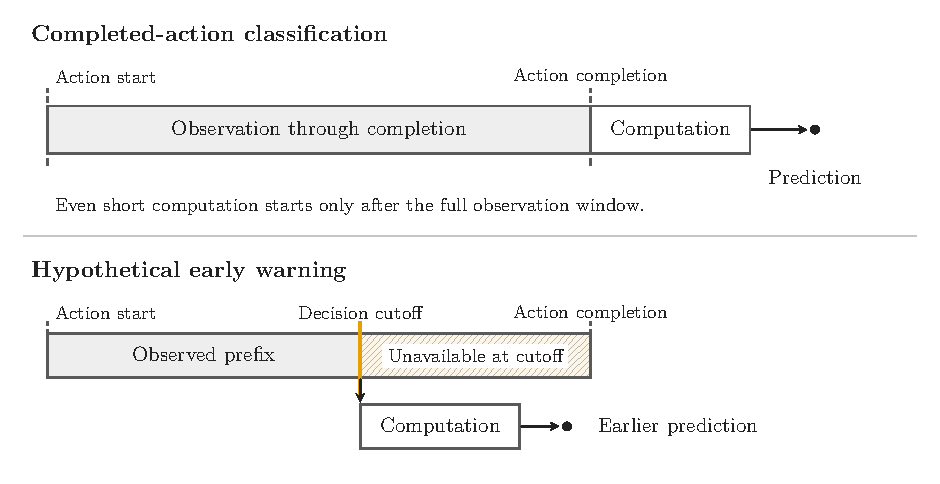
\includegraphics[width=\linewidth]{figures/review_explanatory_20261126/prediction_availability.pdf}
\end{figure}

\section{Multimodal Data in Industrial Applications}

Complementarity is determined by the additional task-relevant information provided by an observation
or representation, rather than by differences in tensor shape or the number of acquisition sources.

Different representations of the same physical quantity can contain complementary information.
Likewise, physically distinct sensors can provide redundant or only very weakly relevant information
for a given prediction target.

The review therefore distinguishes between physical acquisition channels and derived representations
and considers ordinary pairing separately from cases requiring stronger correspondence, such as
cross-modal reconstruction or monitoring of a localised process.

\subsection{Visual and Video Observations}

RGB images, thermal images, process videos and geometric observations all have different acquisition
assumptions. Depth, depth-derived point clouds, and estimated surface normals can all be multiple
views of the same geometric source.

GPAD combines RGB-depth features with point cloud priors \parencite[pp.~4--7]{P024}. This is an
example of integration across representations that do not necessarily require three separate
physical acquisition sources.

RGB-geometry benchmarks describe appearance and shape rather than controller dynamics or motor
current \parencite{Bergmann2022The,Bonfiglioli2023The}.

Physical camera-plus-measurement precedents include thermal imaging with vibration, welding images
with sound, tool images with acoustic emission, and robot video with force/torque and gripper state
\parencite{Huo2022Multisensor,Hua2026Weld,P045,Thoduka2024Handover}.

Their prediction units range from static inspection through to process windows and full trials. In
the tool wear study, the camera is used post-cutting pass, with the preceding acoustic emission
capturing the active cutting \parencite[pp.~19--22]{P045}.

The representation of visual observations also influences the information available. Both pooled
frame features and video Transformers process multiple images, but they differ in how they treat
temporal relationships.

These distinctions between them lead us to explicitly consider visual acquisition, observation
windows, and aggregation within multimodal monitoring architectures.

\subsection{Sensor Time Series and Process Measurements}

Machine measurements can vary enormously in their physical origin and in their semantic meaning. An
accelerometer measures vibration, a pressure sensor measures fluid behaviour, and controller logs
can contain commands, estimates, or tracking errors rather than a direct measure of a physical
quantity.

The harmonic-drive study combines high-frequency vibration with servo information, whereas PGMTKD
transfers pressure-vibration teacher knowledge to a pressure-only student
\parencite{Yang2024Fault,Li2025PGMTKD}.

Both papers address incomplete information, but their sensor availability and deployment reasons
differ.

Representations can also inflate the apparent number of modalities without including any new
measurements. \textcite{Kullu2022A} combine current and vibration using both raw and STFT representations.
\textcite{Wan2024Pipeline} derive statistical 'vibration' features from two acoustic sensors
without acquiring an accelerometer channel at all. \textcite{Wang2025A} combine
source domain features with the decisions from the vibration data.

These studies are useful as architectural comparators, as they examine different information
representations. Their results should, of course, be treated as distinct from comparisons that
incorporate additional physical acquisition sources.

An acquisition inventory and a description of the retained representations are required prior to
attributing any predictive gain to modality diversity.

\subsection{Audio Observations}

Audio can pick up machine/process events that are only very weakly visible. The relationship to
fault state depends heavily on background conditions, mic location, and sync.

MIMII deliberately incorporates factory background recordings at a range of signal-to-noise ratios.
Its fan baseline AUC drops from .94 at $+6$~dB to .70 at $-6$~dB \parencite[Table~3]{Purohit2019MIMII}.

ToyADMOS provides miniature machine recordings and an explicit noise-mixing protocol, making it a
useful reference for acoustic monitoring \parencite{Koizumi2019ToyADMOS}.

In process monitoring, airborne acoustic signals can be paired with either a melt pool camera or a
photodiode. Signal-to-image encoding in the study by \textcite{Li2022A} is an acoustic-optical-signal experiment,
and \textcite{Xie2025Audiovisual} use actual camera images.

DCASE2020 Task2 provides audio-only baselines under an evaluation protocol that differs from that of
later domain shift challenges \parencite{Koizumi2020Description}.

Together, these studies motivate acoustic representations as candidates for industrial multimodal
monitoring. Their utility will depend on the availability of appropriate recordings, well-defined
targets, and correspondence with other observations.

\subsection{Synchronisation, Correspondence, and Modality Availability}

Fusion requires observations that refer to a compatible event, region or time interval. Predicting
one modality from another or combining aligned spatial discrepancy maps requires stronger
correspondence.

RGB-point cloud feature mapping uses registered benchmark geometry. Process monitoring may instead
require time synchronisation and projection onto a common spatial grid
\parencite{Costanzino2024Multimodal,Petrich2021Multimodal}.

In the inspected author manuscript, the digital twin study maps sensor features and prediction
outputs to robot TCP positions. These positions provide spatial registration; they are not among
the 27 listed sensor features \parencite{Chen2023Multisensor}.

Modality availability has several levels. A file can exist without having a usable paired
observation for a given prediction unit. A file can have a successfully paired observation which is
still degraded.

The acoustic-photodiode study explicitly lacks modality registration, which limits claims about
correspondence between its two encoded streams \parencite{Li2022A}.

For camera and machine sensor monitoring, we can have an explicit pairing rule that picks up
unmatched events even if both underlying files are present. Modality completeness should therefore
be assessed on a prediction-unit basis rather than inferred from the presence or absence of the
files.

\section{Representation Learning for Industrial Monitoring}

The choice of representation depends on what an industrial prediction task requires.

The literature reviewed supports both engineered and learned representations. Which is more
appropriate will depend on the level of supervision, the level of preprocessing, the level of
independent sample support, the information required, and the resources available for model fitting.

\subsection{Engineered Features and Conventional Machine Learning}

Engineered summaries impose a constraint on the information that a predictor can use. Measures of
location, spread, amplitude, and trend can describe an operating state without requiring a
high-capacity sequence model to be estimated from a small number of independent observations.

The literature is replete with evidence of compact representations. Hand-crafted local geometry is
competitive in 3D inspection, and a hydraulic CNN paper reports 1.7\% error for its best single
sensor versus 20.5\% error for all seventeen sensors \parencite{Horwitz2023Back,Goodarzi2023Deep}.

These results highlight the necessity for robust conventional references and careful selection of
predictive information.

Industrial vision also offers lightweight alternatives. The weakly supervised inspection network
uses a single camera, internal anomaly-aware features, and a compact CNN. Reported computational
cost is 2.33 million parameters and 5.65~ms per image \parencite[Table~V]{P035}.

The study provides some relevant evidence on representation efficiency, but the anomalous training
labels and modified MVTec supervision differ significantly from normal-only inspection.

Conventional and learned representations should be compared using the same prediction target,
assessment observations, and appropriately fitted preprocessing, rather than ranked solely by model
family.

\subsection{Pretrained Visual Representations}

Pretrained visual representations provide a strong scientific explanation for transferring knowledge
learned from large image collections to industrial applications with far less supervision. The
features they learn may well contain the local appearance, texture, and object configuration
relevant to the downstream prediction task.

PatchCore successfully employs pre-trained, locally aggregated intermediate CNN features together
with a memory of nominal patches for industrial inspection \parencite[Section~3]{Roth2022Towards}.

This provides evidence for investigating transferred spatial representations, though its
nominal-only patch retrieval differs significantly from supervised action classification.

RT-DETR provides another architectural precedent in the form of its multi-scale visual backbone
\parencite[Sections~4.1--4.2]{Zhao2024RTDETR}. Features at several spatial scales would be viable
candidates for the prediction target.

Its published detection accuracy and computational performance pertain to the complete detection
architecture rather than the downstream classification performance of the extracted CNN features.

Asymmetric student-teacher and cross-modal mapping methods also provide further evidence for
task-specific use of the learned visual representations
\parencite{Rudolph2023Asymmetric,Costanzino2024Multimodal}.

Vision-language inspection introduces semantic information as another potential source of
representation value. DSE-AD combines historical and current rail images with normal and abnormal
position prompts and assesses pixel localisation on a further rail domain \parencite{P031}.

Its pair-reference and prompt assumptions differ significantly from those of isolated image
classification.

Together, these studies point to pretrained visual features as plausible candidates, while also
highlighting the need to assess their actual information content, trainable parameters, and
observation horizon in the downstream monitoring task.

\subsection{Temporal and Time-Series Representations}

Temporal representation learning provides an opportunity to retain sequence information that would
otherwise be lost in engineered summaries.

PatchTST addresses this through patch-based time-series representations and shared modelling across
channels \parencite[Sections~3.1--3.2]{Nie2023PatchTST}.

On the Weather dataset at a forecasting horizon of 96, the patch-plus-channel independent model
obtains an MSE of .152, compared with .164 without patching \parencite[Table~7]{Nie2023PatchTST}.

This provides positive evidence for patch-based representation learning in the forecasting setting
under consideration. However, the relevance to industrial classification warrants separate
investigation, as the prediction target, normalisation, supervision, and aggregation differ.

Video representation learning looks at another temporal structure. TimeSformer and Video Swin model
the spatial and temporal relations between video frames \parencite{P034,P013}.

These approaches provide an alternative to simply averaging independently encoded frames. The
industrial CNN-LSTM remaining useful life study also shows the importance of observation length
within its simulated prediction task \parencite{AlDulaimi2019A}.

The literature therefore motivates comparisons that explicitly account for sequence length,
observation windows, temporal ordering, normalisation, pre-training, and fitting budget.

A Temporal Transformer and a compact statistical representation could well be preserving different
aspects of the same sensor stream. Looking at their individual and combined performance helps assess
whether the additional representation contains useful information for the task at hand.

\subsection{Audio Representations}

Acoustic representations include MFCCs, log-mel spectra, wavelet maps, GASF transforms and learned
features.

The Welding Penetration Network uses VMD and GASF; DMAW uses Transformer representations adapted to
the welding observations \parencite{Hua2026Weld,P003}.

These are alternative forms of acoustic representation. An image-shaped acoustic representation is
still one derived from sound rather than being an independently acquired camera stream.

The Audio Spectrogram Transformer is a pretrained candidate for acoustic representation learning
\parencite{P011}. The results on the general audio benchmark are sufficiently promising to warrant
industrial investigation. However, the appropriateness of such representations will depend heavily
on the particular acoustic environment and the specific prediction task.

MIMII and ToyADMOS both go some way to establishing the importance of background composition and
noise environment \parencite{Purohit2019MIMII,Koizumi2019ToyADMOS}.

Together, these studies lead one to consider recording quality, normalisation, and consistent
observation intervals when looking at audio representations.

\subsection{Frozen Representations, Fine-Tuning, and Computational Restrictions}

Freezing an encoder, fitting a small prediction head and then adapting the entire network all
consume different amounts of statistical and computing resources.

Benchmark methods based on pretrained features show that you can get useful representations without
going through the entire original representation-learning process on the industrial dataset
\parencite{Roth2022Towards,Costanzino2024Multimodal}.

The computational cost of pretraining is still part of the representation's provenance even if it's
external to the downstream experiment.

Frozen feature extraction can therefore enable comparisons under a constrained fitting budget.
Fine-tuning provides a very different opportunity in that it allows you to adapt the representations
to the particular target observations. Which of the two is ultimately more effective can only be
determined by empirical comparison, rather than by assuming one approach is in principle better than
the other.

Distillation also makes a further distinction between training and deployment. The PGMTKD multimodal
teachers are used to enrich a pressure-only student. The gated acoustic-vibration study reports a
distilled LightGBM student, though the nature of the teacher features and the timing of the inputs
remain ambiguous \parencite{Li2025PGMTKD,Huang2026Rolling}.

Resource comparisons should therefore account for feature extraction, preprocessing, trainable
components, and any teachers required during inference, rather than just the final prediction model.

These results motivate comparisons of representation and fitting procedures under plausible computing budgets.

\section{Multimodal Fusion Strategies}

Fusion strategies can be broken down according to where the information is fused. Early integration
fuses raw observations or raw features. Intermediate integration fuses the learned representations.
Prediction-level fusion fuses the outputs (e.g., class probability estimates, anomaly scores).
Hybrid architectures use more than one level of integration.

These provide an operational taxonomy for comparing the studies reviewed. Adaptive reweighting
refers to whether the combination varies according to the observation or its context and can
therefore operate at different fusion levels.

Terminology from the source papers is kept where appropriate, and comparisons are based on the
actual location and mechanism of information exchange.

\subsection{Unimodal References and Incremental Modality Value}

The strongest credible single-input predictor provides the reference for measuring the incremental value of fusion.

DMAW fuses the image and
audio Transformer representations to classify the four welding states. The reported accuracy is
96.1\% with fusion, 90.2\% for the image model and 84.4\% for the audio model \parencite[Table~III]{P003}.

This supports a predictive benefit from the assessed multimodal pipeline. The grouping of the
assessment windows by welding run is still not resolved in the evaluation.

In contrast, the weld penetration study reports 100\% clean test accuracy for its image-only,
audio-only, and fused models \parencite[Tables~1--3]{Hua2026Weld}.

The additional modality therefore provides no measurable gain in accuracy under that comparison.

A similar distinction is made in the case of robotic monitoring. The HANDOVER study reports 69.1\%
accuracy for video plus force/torque and 67.9\% when gripper state is added to the I3D-D family
\parencite[Table~III]{Thoduka2024Handover}.

These are five-class outcome accuracies averaged over five training runs. Within that comparison, adding an observation reduced predictive performance.

The tool wear study reports an MAE of 6.6183 for their proposed model, 8.3002 for the visual
ResNet50 and 60.5118 for the acoustic reference. All the other multimodal architectures evaluated
have errors in excess of 45 \parencite[Table~1]{P045}.

The strong visual reference makes the improvement scientifically informative, though the
architectural differences mean you cannot attribute all of it to fusion.

Transferable results on the difficulties of multimodal optimisation and on industrial all-channel
losses underline the need to establish incremental gains against a strong admissible reference
\parencite{Wang2020What,Goodarzi2023Deep}.

Collectively, these studies support investigating the value of conditional fusion, rather than
assuming that including additional modalities will necessarily improve prediction.

\subsection{Feature Concatenation}

Feature concatenation combines the representations with no explicit mechanism for adaptive
allocation and is therefore a key reference point for any more sophisticated form of integration.

Effectiveness depends on feature scale, dimensionality, regularisation, and the quality of the
constituent representations.

M3DM's direct concatenation ablation is worse than its point cloud reference, while the full hybrid
system outperforms both individual inputs \parencite[Table~4]{Wang2023Multimodal}.

MADFlow also provides a further protocol-specific comparison between alignment and concatenation
\parencite{Li2025MADFlow}.

CFA provides transferable evidence from forecasting. For DLinear on the Energy dataset, the first
concatenation gives an MSE of .670, compared with .263 without text and .243 with constrained fusion
\parencite[Table~4]{P023}.

The constrained fusion method also performs worse in a number of the evaluated scenarios, which
again suggests that the benefits of an integration mechanism are highly task-dependent.

Manufacturing fusion can similarly improve one architecture at the expense of the other under the
same broad prediction task \parencite[Table~3]{Li2022A}.

These results establish concatenation as a valid comparator. It should be appropriately normalised
and fitted, rather than implemented as an artificially weak baseline against which more complex
methods are compared.

\subsection{Prediction-Level and Late Fusion}

Prediction-level fusion involves fusing the outputs of modality-specific predictors via techniques
such as averaging, stacking, or evidence aggregation. This is a classification of where the fusion
occurs; the individual predictors could be trained independently or as part of a wider training
regime.

Thermal-vibration diagnosis provides direct evidence of physical camera-sensor prediction-level
fusion. They use separate CNN softmax outputs with weighted Dempster-Shafer aggregation and report a
clean 100\% diagnostic rate, compared with 99.06\% for IRT and 96.32\% for vibration \parencite[Table~VII]{Huo2022Multisensor}.

The weights were fixed, and the sample-level cross-validation did not establish independence between
physical runs.

HANDOVER compares late outputs with intermediate sensor integration in the RGB and optical flow
branches \parencite[Section~IV.A, Figure~3 and Table~III]{Thoduka2024Handover}.

Cross-modal feature mapping and CPIR combine discrepancy maps, which need not be probabilities
\parencite{Costanzino2024Multimodal,Shangguan2025CPIR}.

Some papers also use the term 'late fusion' to describe representation-level integration prior to
classification \parencite{Wang2020What}. That underlines the importance of knowing
what information you are actually fusing.

Stacked generalisation provides a scientific basis for learning a second-stage combination from
cross-validated predictions. Probability outputs contain predictive information beyond the hard
class labels so that a second-stage learner can estimate the joint utility of the outputs
\parencite[Sections~2--3]{Ting1999Issues}.

Ting and Witten fitted a linear least-squares combiner to the class probabilities. A test of such a combination needs predictions for observations held outside the fitting of its component models \parencite[Sections~2--3]{Ting1999Issues}.

\subsection{Gated and Context-Conditioned Fusion}

Adaptive fusion is scientifically justified when the utility of the individual inputs varies from
observation to observation.

Gated Multimodal Units do provide evidence of transferable conditional representation integration.
The architecture fuses visual and textual information and achieves a macro F-score of .541, compared
with .521 for the concatenation baseline in the movie-genre classification task \parencite[Section~3.1, Table~2]{P006}.

The gate in that study operates on learned representations before classification.

Adaptive integration has also been looked at in an industrial context. DMAW achieved 96.1\%
accuracy, compared with 90.5\% for summation and 92.6\% for its gate comparator \parencite[Table~V]{P003}.

TC-MAF provides another approach whereby the auxiliary RGB evidence is bounded around a multimodal
anchor using normal training dispersion and local disagreement \parencite[Section~3.3, Equations~2--4]{P026}.

These architectures illustrate various approaches to controlling information contribution.

An important evaluation dimension is what governs the allocation. GCCF-AD is described as dynamic
fusion, but the formulation they report is a learned scalar with no explicit sample-quality input
\parencite[p.~149226, Equation~8]{P038}.

PGMTKD uses training losses to assign teacher contributions, and task loss balancing focuses on
optimisation rather than any direct measure of input quality at deployment
\parencite{Li2025PGMTKD,P045}.

GAF-Net uses progressive feature feedback, and trustworthy fusion employs evidence-based aggregation
\parencite{Huang2026Rolling,Ying2025Trustworthy}.

The scientific distinction is what contributions can vary, what information determines that
variation, and whether that variation improves predictive performance relative to a fixed
combination.

Process-conditioned weighting provides an additional way to incorporate pertinent context, without
requiring explicit physical law-constrained modelling.

\subsection{Comparability and Fairness of Fusion Evaluations}

A shared dataset name does not in itself constitute a matched experimental comparison.

Cohort construction, supervision, observation windows, pretraining, feature dimensionality,
augmentation, and selection exposure could all contribute to differences between architectures.

The tool wear study alters the architectural components as part of the fusion, and the incomplete
federated imagery study alters the client data access as well as the combining mechanism
\parencite{P045,P051}.

These are comparative assessments of fitted pipelines. Their interpretation differs from an
experiment intended to isolate attention, modality contribution, or quality conditioning.

Comparisons using the same evidence sources can support a narrower attribution. TC-MAF retains the
same evidence sources, comparing bounded fusion against static averaging, weighted scores, rank
fusion, and a learned gate \parencite[Table~3]{P026}.

On the flip side, the disagreement-aware study uses a locally released code baseline that performs
worse than the published M3DM result \parencite[Table~4]{P033}.

Distilled predictors can also access training information that is not available to standard unimodal
models \parencite{Li2025PGMTKD}.

These settings remain scientifically valuable, provided that the information and fitting conditions
are clearly specified. Pipeline performance, incremental modality value, and the isolated effect of
a fusion operator represent distinct evaluation questions.

\section{Reliability and Robustness}

The reliability of a multimodal architecture depends on both the prediction setting and the type of
intervention acting on its inputs.

Missing channels, corrupted measurements, asynchronous observations and changes in operating
conditions all represent different reliability issues. The evidence reviewed is therefore grouped by
the particular condition under consideration rather than assigned to a single general robustness
category.

\subsection{Missing Modalities}

Planned single-input deployment differs from an unannounced loss of an input in a model that
normally expects complete observations.

In the initial appraisal, four of the 37 works examined planned missing-input inference and one examined simulated dropout (five of 37, or 13.5\%, Table~\ref{tab:literature-matrix}). This count combines two missing-input codes. The expanded summary instead records eleven direct tests of missing inputs at inference among 94 appraisals (Figure~\ref{fig:review-depth}); it classifies the depth of evidence rather than the type of absence. The denominators and coding questions therefore differ, and the retained records do not provide a per-work crosswalk between them.

PGMTKD's pressure-only student and incomplete RGB-geometry methods do provide evidence for reduced
input inference. ModDrop and the missing-modality Transformers add further transferable mechanisms
and counterexamples \parencite{Li2025PGMTKD,Sui2026Incomplete,P005,P016}.

The effectiveness of these mechanisms will, of course, depend on the training conditions and the
specific missing-input patterns they have been assessed on.

TC-MAF explicitly evaluates unavailable 3D input. I-AUROC drops from .9788 to .9330 and P-AUPRO from
.9901 to .9586 \parencite[Table~3]{P026}.

This provides a quantified example of performance under a given missing modality condition.

Federated substation monitoring varies the proportion of incomplete clients to 80\% \parencite[Figure~8]{P051}.

Its training and client-availability setting differs from an arbitrary inference-time camera
failure.

ZSG-IAD reports input subset comparisons without fully defining the shared checkpoint and training
exposure \parencite{P025}. Missing training images in the hot rolling regime constitute another
availability regime \parencite{Ma2025A}.

These studies collectively indicate the need to explicitly specify available modalities during both
training and inference (i.e., availability masks), the policy for replacement or fallback, and the
system's response when all required inputs are absent.

\subsection{Noise and Partial Degradation}

Physical monitoring studies do provide evidence of a number of controlled degradation mechanisms.
Thermal-vibration diagnosis examines Gaussian noise and vibration bias/stuck faults, while welding
penetration recognition examines artificial interference. Acoustic-thermal and acoustic-vibration
studies look at other noise settings
\parencite{Huo2022Multisensor,Hua2026Weld,Ying2025Trustworthy,Huang2026Rolling}.

These interventions vary in the observations affected, the degree of corruption and the extent to
which the model is exposed to degradation.

At $-2$~dB, noisy IR thermography gives 95.26\%, which jumps to 97.6\% when combined with fault-free
vibration. Noisy vibration alone gives 36.86\%, jumping to 94.2\% when combined with fault-free IR
thermography \parencite[Table~VIII]{Huo2022Multisensor}.

The comparison shows the value of a fault-free companion modality when another observation is
synthetically corrupted.

The welding penetration study reports a fused accuracy of 93.33\% under its interference condition
\parencite[Table~3]{Hua2026Weld}.

The corresponding corrupted unimodal comparisons are required in order to assess the incremental
benefit of fusion in the interference condition. The reported intervention also leaves some
uncertainty about the corruption operator, magnitude, and exposure matching.

Synthetic signal-to-noise interventions provide some controlled experimental evidence, but the
conclusions are specific to the observations affected and the severities tested. Natural
simultaneous degradation and ordinary defective objects are quite different phenomena.

These distinctions lead directly to a comparison of predictions from degraded input against those
from static fusion and single-input predictors under the same reliability condition.

\subsection{Temporal Misalignment and Distribution Shift}

Temporal misalignment and distribution shift both affect multimodal prediction, albeit in different
ways.

A clock offset can break correspondence between observations, whereas a distribution shift can
change the conditions under which the learned representation or predictor is evaluated.

Registration studies have established the importance of alignment in multimodal monitoring.
OmniFuser's repeated within-pass images provide a way to construct paired observations rather than
directly test a synchronisation failure \parencite{Petrich2021Multimodal,Chen2023Multisensor,P021}.

The literature also contains examples of evaluation under changed acquisition conditions. HANDOVER
trains on one robot and evaluates on a different robot \parencite[Table~V]{Thoduka2024Handover}, and there's a rail localisation study that
evaluates a Subway-trained model on high-speed rail
\parencite[Table~III]{P031}.

Target-adaptive methods, target-validated condition studies and independent build experiments are
all different forms of access to the assessment domain
\parencite{Wang2025A,Chu2024A,Huang2026Rolling,Bevans2023Heterogeneous}.

Rebuilding normal memories on Eyecandies using fixed fusion hyperparameters is evidence of recipe
transfer, rather than deploying an unaltered model to an untouched target installation
\parencite{P026,P033}.

Architecture reuse, representation transfer, temporal offset tolerance, and unchanged-model generalisation each require distinct evaluation protocols.

\subsection{Quality-Aware and Uncertainty-Aware Fusion}

Quality-aware fusion is driven by the idea that the predictive utility of an input may vary with its
quality. Signal quality, model confidence, calibrated probability and evidence consistency are all
distinct concepts.

QMF furnishes a theoretical basis for studying sample-dependent weighting via generalisation upper
bounds under stated relationships between uncertainty and loss, assuming a common training and test
distribution \parencite[Sections~3.1--3.2]{Zhang2023QMF}.

The transferable UDML experiments train on controlled Gaussian corruption intensities and recognise
that sample difficulty can be confused with modality corruption \parencite[pp.~4--5, 9]{P022}.

These results lead us to ask whether the quality information we have available helps us identify
when a particular observation is no longer useful.

QMF reports an NYU scene classification accuracy of 70.09\% on clean inputs, compared to 70.30\% for
concatenation. At corruption intensity ten, it reports 55.60\% compared to 51.99\% for late fusion
\parencite[Table~1]{Zhang2023QMF}.

These non-industrial RGB-depth comparisons do show a regime-specific advantage under corruption. The
clean and corrupted comparisons quoted use different reference methods, so they should not be read
as a clean-versus-corrupted trade-off against the same reference method.

The effect of the adaptation mechanisms also differs across prediction endpoints. The disagreement
add-on increases the local MVTec image AUROC from .779 to .800 and, at the same time, reduces the
Eyecandies image AUROC from .810 to .794, even though the pixel metrics have improved \parencite[Tables~4--5]{P033}.

TC-MAF uses normal-training dispersion and local disagreement to control the contribution of
auxiliary evidence \parencite{P026}.

Collectively, these findings establish a scientific basis for reducing reliance on a stream when the
observable context is expected to indicate errors. They also underscore the need to assess the
relationship between available quality indicators and actual predictive reliability.

QMF's theoretical justification does not validate the use of arbitrary quality proxies, and clean
calibration can actually degrade after a distribution shift \parencite{Zhang2023QMF,P008}.

For quality-conditioned weighting, the relevant comparison is with a static model given the same training exposure to corruption. Performance on clean observations also matters.

\subsection{Modality Dropout, Augmentation, and Fallback Mechanisms}

Different robustness mechanisms deal with different aspects of input availability.

Training-time modality dropout exposes the model to certain absence patterns. Imputation produces
substitute observations, and deterministic fallbacks route the prediction to an available unimodal
component.

These approaches can generate similar outputs under certain conditions without relying on the same
learned recovery mechanism.

The fuzzy-regularisation study introduces failures via partial corruption and by replacing the
entire input with a constant or noise. The evaluation is of Gazebo pose regression using random
sample splits of overlapping windows \parencite[Sections~III.A and IV.A--IV.B]{Altinses2023Fuzzy}.

The investigation provides evidence for controlled input regularisation, with independent physical
deployment outage performance remaining unaddressed.

OmniFuser describes dropout and masking without any quantified outage table \parencite[p.~10]{P021}.

Generated replacement observations can also have a negative impact on performance. Replacing the
clean depth with CycleGAN output worsens the synthetic robot benchmark's MSE (from $2.1745 \times
10^{-3}$ to $13.472 \times 10^{-3}$) \parencite[Table~7]{Altinses2025Performance}.

These results motivate individual evaluation of learned recovery, training exposure, and explicit
fallback policies. Static controls, with equivalent degradation exposure and predictions from the
surviving input, provide a useful baseline for assessing adaptive robustness.

\section{Evaluation Beyond Accuracy}

The practical value of a monitoring architecture will depend entirely on how its predictions are
evaluated, chosen, and interpreted.

Accuracy in prediction can be affected by class distribution, assessment grouping and decision
thresholds. A single aggregate score therefore only provides one facet of the evidence needed to
assess the performance of a multimodal industrial monitoring system.

The evaluation questions concern assessment independence, discrimination, calibration, uncertainty, interpretability, computational viability and reproducibility.

\subsection{Grouped Evaluation and Leakage Prevention}

The independent assessment unit may be a weld, a tool, a participant, a recording, a machine or a
build.

Randomly partitioned observations can end up with shared acquisition contextual information or raw
samples. The fuzzy-regularisation study forms 20-step windows with a stride of one and reports a random
division of the samples \parencite[Sections~IV.A--IV.B]{Altinses2023Fuzzy}.

Its assessment therefore doesn't establish performance on unseen trajectories.

Weld run grouping is still unresolved in the closest welding studies \parencite{P003,Hua2026Weld}. These
examples do show a potential dependence between the observations but do not establish any particular
level of leakage.

The HANDOVER authors report an explicit participant-disjoint official split \parencite{Thoduka2024Handover}.

Normalisation, feature selection and model parameter optimisation all require an appropriate split
between model development and model assessment \parencite{P004,P017}.

Out-of-fold stacking provides a mechanism for constructing second-stage prediction inputs without
any in-sample predictions. Its validity is of course also dependent on the way in which the
underlying fitting, selection and calibration folds are constructed.

Repeatedly selecting follow-up experiments after looking at the assessment results introduces
further selection bias, even if the individual model fits would have ruled out their outer test
labels.

These results motivate the development of assessment protocols that account for the physical origin
and dependence of observations throughout the modelling process.

\subsection{Discrimination, Calibration, and Decision Thresholds}

Ranking, probability quality and thresholded decisions are three different aspects of a predictor.

AUROC measures discrimination across thresholds rather than performance at a single operational
false alarm rate or the quality of the predicted probabilities.

MVTec AD shows that useful ranking can exist alongside fairly poor thresholded localisation. The
strict FPR metrics highlight a different aspect of detection performance
\parencite{Bergmann2019MVTec,Costanzino2024Multimodal,Cheng2025Multimodal}.

The rail vision-language study reports pixel-level metrics and optimal threshold F1 score \parencite[Section~IV.B.2]{P031}. These metrics address a completely different evaluation problem than image-level alarm
accuracy at a threshold chosen from the training or validation set.

In manufacturing, \textcite{Petrich2021Multimodal} report an accuracy of .9921 and a precision of .2487 on an
imbalanced layer, which is a clear example of the impact of class distribution and threshold
selection.

Validation-fitted calibration can improve in-distribution probability quality, while dataset shift
can damage confidence estimates \parencite{Guo2017Calibration,P008}.

Proper scoring rules (negative log-likelihood, Brier score, etc.) provide a basis for assessing
probability forecasts \parencite{P055}. Their interpretation differs from that of discrimination or
thresholded classification.

A generated confidence field or evidence mass cannot replace probability evaluation. Metrics should
align with the prediction target and class distribution, and operational thresholds should be
selected using admissible training or validation observations.

\subsection{Uncertainty and Statistical Comparisons}

Seed variation, acquisition group sampling and model selection uncertainty are all different sources
of variation.

HANDOVER's reported standard deviations are for five training runs on a fixed test set, whereas a
group bootstrap of saved predictions samples assessment units conditional on the fitted models
\parencite{Thoduka2024Handover}.

These approaches capture different facets of uncertainty and do not necessarily encompass all the
variation expected from retraining or deployment in a different domain.

Cross-validation folds share training observations. Under the assumptions stated, the classic
variance result shows that no universally unbiased estimator of cross-validation variance exists;
ignoring covariance can substantially underestimate uncertainty \parencite[pp.~1096--1098, 1102--1104]{Bengio2004CVVariance}. Conditional uncertainty intervals can still be useful when the
estimand and dependence assumptions are stated explicitly.

Small fusion effects, ambiguous repetition counts and conflicting descriptions of significance all
warrant the same level of caution \parencite{Gu2024Improved,Xu2025ModalityResilient}.

Paired performance differences on common assessment observations provide a much more direct
comparison than unrelated score intervals. An interval which contains zero doesn't demonstrate
equivalence, and a positive point estimate doesn't establish practical importance without an
appropriate criterion.

\subsection{Interpretability and Its Limits}

Prediction scores, coefficients, gate traces and spatial maps can all tell you something regarding
how the model is behaving.

The attention debate has both counterexamples to faithful explanation and evidence that the learned
attention weights do, in fact, contain useful information. This leads to the conclusion that
interpretability should be evaluated on a task-specific basis rather than drawing general
conclusions from the terminology of the architecture itself \parencite{P036}.

ZSG-IAD measures schema validity, language consistency and coarse-to-final-mask overlap
\parencite{P025}. These provide evidence of various forms of self-consistency.

Their interpretation differs from both independent physical defect causation and calibrated
confidence.

HANDOVER leaves the use of human action prediction as a means of explanation as a future area of
research \parencite{Thoduka2024Handover}.

Describing which signals a model used leaves two further questions open: whether they explain the physical cause and whether the explanation helps an operator make a decision.

Process context should be distinguished from the explicit physical equation constraints \parencite[e.g.,
PGMTKD's pressure model;][]{Li2025PGMTKD}.

\subsection{Modularity, Reproducibility, and Computational Cost}

Modular architectures enable the replacement and comparison of individual representations
and prediction components. Their value for scientific investigation comes from the fact that you
can identify which component is different between conditions.

Modularity does not establish predictive robustness or an advantage over a matched end-to-end
architecture.

An identified version, accessible source code, executable processing and independently reproduced
results all provide various levels of reproducibility assurance \parencite{P009}.

The difference between local and published M3DM results remains unresolved. It motivates checks of
dependencies, valid point filtering, checkpoints, and scoring conventions \parencite{P033}.

Computational comparisons of course also require a common measurement boundary. The CPIR paper
reports lower FPS than CFM, which is a clear performance vs speed trade-off
\parencite{Shangguan2025CPIR}.

The reported 5.65~ms for the lightweight image network doesn't include the independent sensor branch
or acquisition delay \parencite[Table~V]{P035}.

TimeSformer's compute requirements depend on the ImageNet pretraining and the workload it is
evaluated on \parencite{P034}.

Hardware, batch size, caching, synchronisation and the processing stages included all determine
which computational measurements can be compared.

These results indicate the necessity for explicit resource accounting and reproducibility
documentation. Prospective deployment and operator usability remain open questions for validating a
successful offline forward pass.

\section{Critical Synthesis and Research Gap}

The reviewed literature shows that multimodal observations and learned representations can benefit
industrial and robotic monitoring. Their value, however, depends on the prediction task, the
information each representation contains, and the conditions under which the integration method is
evaluated.

The previous sections have identified four related scientific questions: which representations are
appropriate for a given target, whether combining their predictions is valuable, whether that value
is maintained as observation quality degrades, and how the experimental assessments should be
conducted.

\subsection{Findings Supported Across the Reviewed Studies}

There are tangible observations that can be used to improve the performance of a task-specific
monitoring pipeline. DMAW, thermal-vibration diagnosis, HANDOVER and tool wear prediction are all
good examples under their respective assessment protocols
\parencite{P003,Huo2022Multisensor,Thoduka2024Handover,P045}.

Controlled evidence integration can also improve RGB--geometry inspection under intact-input
conditions. TC-MAF separately reports performance when the 3D input is unavailable \parencite{P026}.

The literature therefore establishes that useful industrial multimodal fusion mechanisms and
approaches to dealing with incomplete observations do in fact exist.

Representation learning offers a number of scientifically sound options for extracting information
relevant to the task. Pretrained convolutional features, patch-based temporal representations, and
hand-crafted features are all candidates with some supporting evidence under certain learning and
evaluation regimes \parencite{Roth2022Towards,Nie2023PatchTST,Horwitz2023Back}.

Their suitability for another industrial prediction target will, of course, depend on several
factors, including the observations, the supervision, the aggregation, and the compute resources
involved.

Static and learned fusion mechanisms both offer different avenues for exploiting complementary
information. Stacked generalisation motivates learning combinations of the outputs of individual
predictors. In contrast, gated representation learning and quality-aware fusion justify
context-dependent allocation \parencite{Ting1999Issues,P006,Zhang2023QMF}.

A further well-established distinction concerns input reliability. Planned single-input deployment,
complete inference-time absence, controlled corruption, and target domain adaptation all address
different issues \parencite{Li2025PGMTKD,Altinses2023Fuzzy,P051}.

The consistent finding across the reviewed studies is a conditional benefit under specific tasks and
evaluation regimes, rather than universal superiority of any single representation or fusion
architecture.

Figure~\ref{fig:review-depth} distinguishes a recorded direct test from the use or discussion of a
topic. In this summary, 46 of 94 appraisals record a direct test of adding an input, 21 of
corrupted inputs at test, and eleven of missing inputs at inference; these count the
questions tested, not findings of a benefit.
% The aggregate counts agree with figures/review_figure_table.tex and the 94-work
% corpus register. A per-work crosswalk for the direct-test coding was not retained
% in the inspected appraisal files; this check did not independently recode them.
Training strategy illustrates this distinction: 60 of the 94 appraisals described or used the
training strategy without a recorded direct test, while 28 (29.8\%) recorded a direct test. These
counts describe the depth documented in the appraisals; low frequency alone does not establish
research priority.

\ReviewDepthFigure

\subsection{Unresolved Questions and Research Gap}

The evidence reviewed also contains significant negative and, indeed, conflicting findings.

The same clean-test accuracy is observed for the unimodal and fused welding models. HANDOVER
performance drops when the gripper state is added. Some alternative multimodal tool-wear models
perform worse than the visual reference, although the proposed model improves on it. The Eyecandies
image scores also go down. All of this calls into question the notion of an unqualified fusion
benefit \parencite{Hua2026Weld,Thoduka2024Handover,P045,P033}.

Category-specific geometry losses, poor hydraulic channel combinations, and the difficulties of
multimodal optimisation all reinforce this conclusion
\parencite{Horwitz2023Back,Bonfiglioli2023The,Goodarzi2023Deep,Wang2020What}.

Several mechanisms could account for these results: redundancy, inappropriate representations,
optimisation difficulties, noise, supervision and limited independent sample support. The studies do
not point to a single underlying explanation.

An important unresolved issue is the distinction between a representation's standalone strength and
its complementary predictive value. A representation that is weak in isolation may still provide
information useful for another predictor. Conversely, a strong additional representation does not
guarantee that a fusion mechanism can effectively utilise that information.

Reliability introduces a related source of uncertainty. Adaptive weighting is justified when the
available context can identify changes in unimodal prediction reliability \parencite{Zhang2023QMF,P022}.
The value of conditioning information, its relationship to branch errors, and its comparison with
exposure-matched static alternatives must be investigated on a task-specific basis.

External evaluation adds another boundary. Re-using a procedure with a new dataset-specific fitting,
re-using the learned representation weights and then evaluating an unaltered predictor in a
different domain are all different experimental questions. You cannot just take the results of one
and treat them as equivalent evidence of generalisation.

\section{Final Summary of the Literature Review}

The 94 appraised works support a conditional benefit from multimodal monitoring. In four-state welding classification, combining image and audio raised accuracy from 90.2\% for the stronger single input to 96.1\%. In weld-penetration classification, both individual inputs and their combination reached 100\% on the clean test set \parencite{P003,Hua2026Weld}. In human--robot handover, adding gripper state to video and force/torque reduced five-class accuracy \parencite{Thoduka2024Handover}. Taken together, these comparisons locate the architectural question more precisely: for a given target and observation window, when does a second input retain complementary information, and when does a learned fusion rule use it more effectively than a strong single predictor or a fixed combination under the same fitting and reliability conditions?

\ReviewFollowupTable
